\documentclass{article}

\usepackage[T1]{fontenc}
\usepackage[UTF8]{inputenc}
\usepackage[polish]{babel}

\usepackage{enumitem}
\usepackage{tabulary}
\usepackage{multirow}
%\usepackage{array}
\usepackage{graphicx}
\usepackage{colortbl}
\usepackage{listings}
\usepackage{color}

\definecolor{gray}{rgb}{0.4,0.4,0.4}
\definecolor{darkblue}{rgb}{0.0,0.0,0.6}
\definecolor{cyan}{rgb}{0.0,0.6,0.6}

\lstset{
  basicstyle=\ttfamily,
  columns=fullflexible,
  showstringspaces=false,
  commentstyle=\color{gray}\upshape
}

\lstdefinelanguage{XML}
{
  morestring=[b]",
  morestring=[s]{>}{<},
  morecomment=[s]{<?}{?>},
  stringstyle=\color{black},
  identifierstyle=\color{darkblue},
  keywordstyle=\color{cyan},
  morekeywords={xmlns,version,type}% list your attributes here
}

\let\oldsection\section
\renewcommand\section{\clearpage\oldsection} %break after every section

\definecolor{hlinecolor}{gray}{0.8}

\newcommand{\pielat}{\small{\textsf{MP}}}
\newcommand{\kowalik}{\small{\textsf{WK}}}
\newcommand{\miskiewicz}{\small{\textsf{KM}}}
\newcommand{\everyone}{\small{\textsf{ALL}}}

\begin{document}
\title{\textbf{Projekt Zespołowy}\\Edytor pojazdów i map}
\author{Wojciech Kowalik, Konrad Miśkiewicz, Mateusz Pielat}
\maketitle


\section{XML - do dodania gdzieś}

\lstset{
  language=XML,
  morekeywords={encoding,
    }
}
\begin{lstlisting}
<vmd xmlns="pl.pw.mini.KowMisPie.SRL" width="512" height="512">
  <polygon>
        <point x = "160" y="119" />
        <point x = "58" y="284" />
        <point x = "357" y="275" />
    </polygon>
    <polygon>
        <point x = "393" y="32" />
        <point x = "390" y="398" />
        <point x = "457" y="400" />
        <point x = "458" y="33" />
    </polygon>
    <polygon>
        <point x="233" y="327" />
        <point x="30" y="316" />
        <point x="27" y="60" />
        <point x="357" y="60" />
        <point x="362" y="23" />
        <point x="466" y="21" />
        <point x="467" y="7" />
        <point x="16" y="42" />
        <point x="15" y="334" />
        <point x="258" y="406" />
        <point x="315" y="358" />
    </polygon>
</vmd>
\end{lstlisting}

\begin{lstlisting}
<vvd xmlns="pl.pw.mini.KowMisPie.SRL">
    <orientation>
        <point x="0" y="0" />
        <angle>1.9091524329963763</angle>
    </orientation>
    <polygon>
        <point x="112" y="93" />
        <point x="359" y="95" />
        <point x="433" y="165" />
        <point x="371" y="222" />
        <point x="111" y="222" />
    </polygon>
</vvd>
\end{lstlisting}

\section{Połączenie technologii WPF i MonoGame}

Aby interfejs użytkownika był możliwie prosty, a tworzenie map i pojazdów maksymalnie wydajne połączone zostały technologie Windows Presentation Foundation (WPF) i MonoGame. Technologia WPF domyślnie nie umożliwia osadzenia zewnętrznego silnika graficznego, więc aby móc skorzystać z MonoGame w tym środowisku konieczne było napisanie odpowiedniej kontrolki. 

~\\W związku z tym stworzona została kontrolka \textit{MonoGameControl}. W rzeczywistości jest ona klasą abstrakcyjną, która zawiera trzy metody abstrakcyjne. Aby z niej skorzystać konieczne jest utworzenie własnej klasy dziedziczącej po \textit{MonoGameControl} i implementującej metody: \textbf{Initialize()}, \textbf{Uninitialize()} oraz \textbf{Render(TimeSpan time)}. Budowę takiej kontrolki oraz jej implementację przedstawiono poniżej.

\subsection{Schemat kontrolki hostującej MonoGame}

\begin{center}
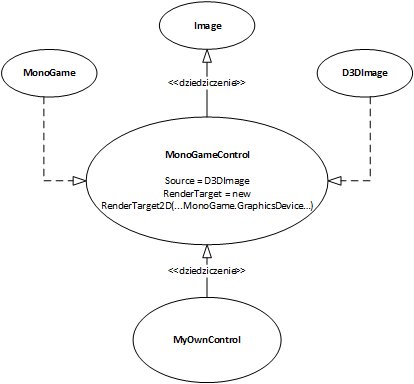
\includegraphics[scale=1.0]{MonoGameControlSchemat}\\
\textit{Schemat 1. MonoGameControl}
\end{center}
~\\
\subsection{Metody abstrakcyjne wymagające nadpisania}
\begin{itemize}
  \item \textbf{abstract void Initialize()} - wywoływana przy tworzeniu kontrolki
  \item \textbf{abstract void Unitialize()} - wywoływana przy destrukcji kontrolki
  \item \textbf{abstract void Render(TimeSpan time)} - wywoływana cyklicznie, odpowiada za ponowne renderowanie obrazu wyświetlanego na kontrolce
\end{itemize}

\subsection{Przykład Implementacji własnej kontrolki hostującej MonoGame}
\begin{lstlisting}
       public class MyOwnControl : MonoGameControl
       {
           private SpriteBatch spriteBatch;
    
           protected override void Initialize()
           {
               spriteBatch = new SpriteBatch(GraphicsDevice);
           }

           protected override void Unitialize()
           {
               spriteBatch.Dispose();
           }

           protected override void Render(TimeSpan time)
           {
               GraphicsDevice.Clear(Color.LightSkyBlue);
               GraphicsDevice.RasterizerState = RasterizerState.CullNone;

               spriteBatch.BeginDraw();

               // DRAW

               spriteBatch.End();
           }
       }
\end{lstlisting}

\section{Osadzenie obrazka}

\begin{center}
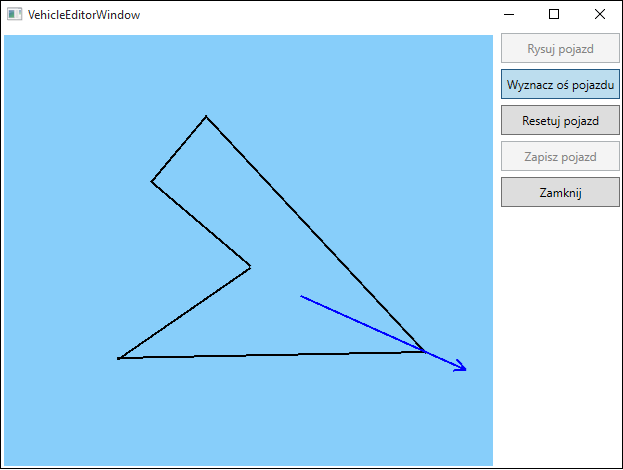
\includegraphics[scale=0.7]{vehicleeditor}\\
\textit{Rysunek 1. Edytor pojazdu}
\end{center}

\begin{center}
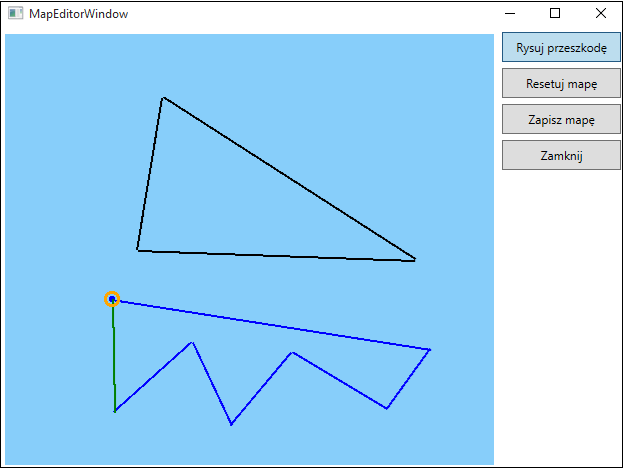
\includegraphics[scale=0.7]{mapeditor}\\
\textit{Rysunek 2. Edytor map}
\end{center}

\subsubsection{Moduł wizualizacji}
\begin{itemize}
  \item System powinien umożliwiać wczytywanie uprzednio zapisanych w odpowiednim formacie map i pojazdów.
  \item System powinien umożliwiać ustawienie początku i końca trasy pojazdu.
  \item System powinien umożliwiać ustawienie prędkości animacji ruchu pojazdu.
  \item System powinien umożliwiać pauzowanie trwającej wizualizacji.
  \item System powinien umożliwiać przejście suwakiem do dowolnego momentu symulacji.
  \item System powinien umożliwiać zapisywanie wygenerowanej symulacji.
\end{itemize}

\subsubsection{Moduł rysowania pojazdów i map}
\begin{itemize}
  \item System powinien umożliwiać rysowanie wielokątów reprezentujących pojazdy lub przeszkody omijane przez pojazd.
  \item System powinien zamykać wielokąt, jeżeli użytkownik nie zamknie go sam.
  \item System powinien umożliwiać zapisywanie narysowanych pojazdów/map do postaci wektorowej.
\end{itemize}

\subsubsection{Moduł generowania pojazdów i map z plików graficznych}
\begin{itemize}
  \item System powinien umożliwiać wczytanie pliku graficznego w jednym z dozwolonych formatów.
  \item System powinien umożliwiać dobór parametrów trasowania.
  \item System powinien wyświetlać użytkownikowi wynik trasowania dla aktualnie dobranych parametrów.
  \item System powinien umożliwiać zapisywanie wygenerowanych pojazdów/map do postaci wektorowej.
\end{itemize}

\subsubsection{Moduł algorytmu}
\begin{itemize}
  \item System powinien znajdować ścieżkę między punktem startowym a punktem końcowym dla danego pojazdu z uwzględnieniem przeszkód.
  \item System powinien eksportować wynik obliczeń do listy rozkazów.
\end{itemize}


\section{Wymagania niefunkcjonalne}

\begin{itemize}
  \item Aplikacja powinna poprawnie działać na systemach operacyjnych z rodziny \textit{Windows}.
  \item System powinien poinformować użytkownika, gdy przeprowadzenie symulacji jest niemożliwe.
  \item Dozwolone formaty dla plików graficznych: \textbf{bmp}, \textbf{jpeg}, \textbf{png}, \textbf{gif}.
  \item Rysowanie pojazdów i map nie powinno odbywać się poprzez rysowanie ciągłe, a raczej poprzez dodawanie kolejnych punktów do wielokątów.
  \item Podczas rysowania wielokątów ich krawędzie nie mogą się przecinać. 
  \item System powinien dać się łatwo tłumaczyć na różne języki:
  \begin{itemize}
    \item Powinien mieć wbudowany język polski i angielski.
    \item Dodanie nowego języka powinno ograniczać się do zmian w pliku konfiguracyjnym.
  \end{itemize}
\end{itemize}


\section{Metodologia pracy}

Aplikacja będzie tworzona zgodnie z modelem przyrostowym (ang. \textit{incremental development}). Zakłada on realizację jedynie pewnej części systemu w każdym kolejnym `cyklu pracy. Poszczególne porcje funkcjonalności powinny być spójne, aby możliwe było przetestowanie i dostarczenie ich w wersji finalnej klientowi.

\subsection{Uzasadnienie wyboru}

Preferencja modelu przyrostowego nad modelem kaskadowym wynika ze struktury naszej aplikacji. Można ją podzielić na wiele odrębnych modułów działających (do pewnego stopnia) oddzielnie i niezależnie od siebie. Ponadto, ta metodologia zakłada brak konieczności definiowania z góry szczegółowych wymagań poszczególnych części systemu, dzięki czemu proces tworzenia jest bardziej elastyczny niż w przypadku modelu kaskadowego.

\section{Harmonogram pracy}
\setlist{nosep}
\begin{tabulary}{\textwidth}{cp{0.8\textwidth}c}
  \arrayrulecolor{hlinecolor}\hline
 
  %-------------------------------------------------------------
  \hline
  & & \parbox[t]{2mm}{\multirow{13}{*}{\rotatebox[origin=c]{-90}{17.11.15}}} \\ 
  \multicolumn{2}{l}{\textbf{Architektura systemu}} & \\ 
  
  \kowalik & repozytorium i struktura katalogów & \\
  \miskiewicz & przygotowanie diagramu klas & \\
  \everyone & zdefiniowanie reprezentacji pojazdu i mapy & \\
  \everyone & zdefiniowanie reprezentacji rozkazów ruchu pojazdu & \\

  %-------------------------------------------------------------
  \\ \multicolumn{2}{l}{\textbf{Interfejs graficzny}} & \\
  
  \pielat & przygotowanie mock-up poszczególnych okien interfejsu & \\
  \miskiewicz & implementacja interakcji pomiędzy oknami & \\
  
  %-------------------------------------------------------------
  \\ \multicolumn{2}{l}{\textbf{Tworzenie pojazdów i map}} & \\
  
  \miskiewicz & serializacja i deserializacja do XML & \\
  \kowalik & tworzenie pojazdów i przeszkód przy pomocy kursora & \\
  \hline
  \pielat & selekcja trasowanych grafik rastrowych pod względem rozszerzeń i treści & \parbox[t]{2mm}{\multirow{5}{*}{\rotatebox[origin=c]{-90}{01.12.15}}}\\
  \pielat & trasowanie z użyciem wybranej biblioteki; wyświetlanie efektu użytkownikowi dla odpowiednio dobranych parametrów trasowania & \\
  \hline

  %-------------------------------------------------------------
   & & \parbox[t]{2mm}{\multirow{11}{*}{\rotatebox[origin=c]{-90}{15.12.15}}} \\
  \multicolumn{2}{l}{\textbf{Mock-up algorytmu}} & \\
  
  \miskiewicz & losowe generowanie tras & \\
  \miskiewicz & eksport trasy do listy rozkazów & \\
  
  %-------------------------------------------------------------
  \\ \multicolumn{2}{l}{\textbf{Wizualizacja}} & \\
  
  \kowalik & tworzenie przeszkód i pojazdu na mapie & \\
  \kowalik & ustawianie początku i końca trasy & \\
  \pielat & animacja ruchu na podstawie rozkazów & \\
  \miskiewicz & selekcja trasowanych grafik rastrowych pod względem rozszerzeń i treści & \\
  \pielat & implementacja suwaka osi czasu wizualizacji & \\
  \hline
  
  %-------------------------------------------------------------
  & & \parbox[t]{2mm}{\multirow{5}{*}{\rotatebox[origin=c]{-90}{12.01.16}}} \\ 
  \multicolumn{2}{l}{\textbf{Algorytm}} & \\
  
  \everyone & opracowanie koncepcji algorytmu wyszukiwania drogi & \\
  \everyone & implementacja algorytmu wyszukiwania drogi & \\
  \everyone & eksport i mapowanie wyników obliczeń do listy rozkazów & \\
  \hline

\end{tabulary}\\\\
\everyone \space - zadania przydzielone dla wszystkich\\
\kowalik \space - zadania przydzielone dla Wojciecha Kowalika\\
\miskiewicz \space - zadania przydzielone dla Konrada Miśkiewicza\\
\pielat \space - zadania przydzielone dla Mateusza Pielata


\section{Kamienie milowe}

Każdy kamień milowy stanowi oddzielny, funkcjonalny moduł systemu. Wszystkie z nich kończą się testami i dokumentacją.

\setlist{}

\begin{enumerate}
  \item \textbf{Moduł tworzenia map i pojazdów przez użytkownika}\par 
  Zostanie stworzony interfejs użytkownika oraz możliwe będzie ręczne tworzenie map i pojazdów z wykorzystaniem wbudowanego edytora i zapisywanie ich do formatu wektorowego
  \item \textbf{Moduł wczytywania map i pojazdów z plików graficznych}\par
  Możliwe będzie wczytywanie pojazdów i map z plików graficznych oraz eksportowanie ich do formatu wektorowego
  \item \textbf{Moduł wizualizacji ruchu}\par
  Użytkownik może wybierać pojazd, mapę oraz zaznaczać początek i koniec trasy. Mock-up algorytmu wygeneruje losową trasę dla pojazdu, która zostanie przedstawiona użytkownikowi. Użytkownik będzie miał możliwość ustawienia prędkości symulacji, pauzy oraz przejścia w czasie suwakiem.
  \item \textbf{Moduł algorytmu wyszukiwania drogi}\par
  Zaimplementowany zostanie algorytm wyznaczania drogi, który zastąpi wcześniejszy mock-up. Wszystkie moduły aplikacji zostaną ze sobą zintegrowane.
\end{enumerate}

\end{document}